\documentclass[a4paper]{extarticle}
\usepackage{ctex}
\usepackage{titlesec}
\usepackage{lipsum}
\usepackage{geometry}
\usepackage{amsmath}
\usepackage{biblatex}
\usepackage{booktabs}
\usepackage{caption}
\usepackage{graphicx}
\usepackage{float}
\usepackage{subfig}
\setCJKmainfont{STSong}[AutoFakeBold,AutoFakeSlant]
\setCJKsansfont{Microsoft YaHei}
\setCJKmonofont{KaiTi}
\setmainfont{Times New Roman}
\setsansfont{Times New Roman}
\setmonofont{Times New Roman}
\linespread{1.5}
\setlength{\parindent}{0pt}
\titleformat{\section}{\bfseries\fontsize{14pt}{\baselineskip}\selectfont}{\thesection}{0.5em}{}
\titleformat{\subsection}{\bfseries\fontsize{10.5pt}{\baselineskip}\selectfont}{\thesubsection}{0.5em}{}
\titleformat{\subsubsection}{\fontsize{10.5pt}{\baselineskip}\selectfont}{\thesubsubsection}{0.5em}{}
\geometry{left=2.5cm,right=2.5cm,top=2.5cm,bottom=2.5cm}
\everymath{\displaystyle}

\begin{document}
    \begin{center}
        \textbf{\fontsize{22pt}{\baselineskip} \selectfont 液体表面张力系数测定}\\
        \vspace{2em}
        \texttt{\fontsize{14pt}{\baselineskip} \selectfont 作者:刘子墨,学号:PB23000233}\\
    \end{center}
    \vspace{2em}
    \hspace{2em}\textsf{\fontsize{9pt}{\baselineskip} \selectfont 摘要:}
    \texttt{\fontsize{9pt}{\baselineskip} \selectfont 本文通过焦利氏秤法测量了自来水和洗洁精溶液的表面张力系数。最终测得自来水的表面张力系数为$6.09\times10^{-2}$ N/m,其标准不确定度为$1.0\times10^{-3}$ N/m,展伸不确定度为$2.5\times10^{-3}$ N/m;待测洗洁精溶液的表面张力为$2.94\times10^{-2}$ N/m。并对不同浓度洗洁精的表面张力测量,绘制了洗洁精溶液表面张力随浓度变化的曲线。实验结果表明,在测量区间内洗洁精溶液的表面张力随浓度有微弱上升趋势,这可能由洗洁精溶液的浓度较大以及测量区间过小导致。}
    \par\hspace{2em}\textsf{\fontsize{9pt}{\baselineskip} \selectfont 关键词:}
    \texttt{\fontsize{9pt}{\baselineskip} \selectfont 表面张力;焦利氏秤法;不确定度分析}\\ 
    \section{引言}
    \hspace{2em}
    液体具有尽量缩小其表面的趋势,好象液体表面是一张拉紧了的橡皮膜一样。把这种沿着表面的、收缩液面的力称为表面张力。液体表面层(其厚度等于分子的作用半径)内的分子所处的环境跟液体内部的分子是不同的。表面层内的分子合力垂直于液面并指向液体内部,所以分子有从液面挤入液体内部的倾向,并使液体表面自然收缩,从而产生了表面张力。表面张力的存在能说明物质处于液态时所特有的许多现象,比如泡沫的形成、润湿和毛细现象等等。表面张力大小与表面张力系数$σ$和分界线的长度$L$成正比:
    \begin{equation}
        F=\sigma L
    \end{equation}
    式中$\sigma$称为表面张力系数,它的大小与液体的成分、纯度、浓度以及温度有关。
    \par\hspace{2em}
    测定液体表面张力的方法很多,常用的有焦利氏秤法(拉脱法)、毛细管法、平板法、滴重法、最大泡压法等。本实验采用焦利氏秤法(拉脱法)。该方法的特点是,用秤量仪器直接测量液体的表面张力,测量方法直观,概念清楚。
    \section{实验内容与设计}
    \subsection{实验装置}
    \hspace{2em}
    焦利氏秤、钢尺、金属圈、金属丝、砝码、镊子、针筒等。
    \par\hspace{2em}
    焦利氏秤装置如图\ref{fig:1}所示。焦利氏秤是一种用于测微小力的精细弹簧秤。一般的弹簧秤都是弹簧秤上端固定,在下端加负载后向下伸长,而焦利秤与之相反,它是控制弹簧下端的位置保持一定,加负载后向上拉动弹簧确定伸长值。为了保证弹簧下端的位置是固定的,必须三线对齐,即玻璃圆筒上的刻线、小平面镜上的刻线、上的刻线在小平面镜中的像三者始终重合。在力$F$作用下弹簧伸长$\Delta l$,根据虎克定律可知,在弹性限度内$F = k \Delta l$,将已知重量的砝码加在砝码盘中,测出弹簧的伸长量,由上式即可计算该弹簧的$k$值,由$k$值就可测外力$F$。
    \begin{figure}[H]
        \centering
        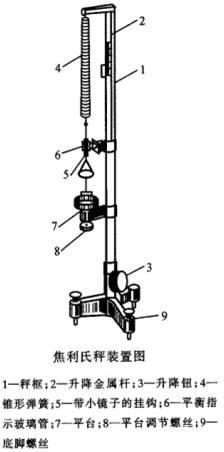
\includegraphics[width=0.3\linewidth]{jiaolishi.png}
        \caption{焦利氏秤装置示意图}
        \label{fig:1}
    \end{figure}
    \subsection{实验方案与设计}
    \hspace{2em}
    金属丝框缓慢拉出水面过程中,金属丝或金属圈下面将带起一水膜,当水膜刚被拉断时,诸力的平衡条件是:
    \begin{equation*}
        F=mg+2F'
    \end{equation*}
    其中$F'=\sigma l$是表面张力的大小,$l$是金属丝或金属圈的周长,$\sigma$是表面张力系数。由此可得:
    \begin{equation}
        \sigma=\frac{F-mg}{2l}
    \end{equation}
    在实际实验中,$F-mg$是金属丝浸入水中时和水膜恰好破裂时弹簧的弹力差,可以通过焦利氏秤弹簧的伸长量变化测量;$l$是金属丝或金属圈的周长,可以通过钢尺测量。
    \subsection{实验内容}
    \subsubsection{确定焦利氏秤上锥形弹簧的劲度系数}
    \begin{enumerate}
        \item 把锥形弹簧,带小镜子的挂钩和小砝码盘依次安装到秤框内的金属杆上。调节支架底座的底脚螺丝,使秤框竖直,小镜子应正好位于玻璃管中间,挂钩上下运动时不致与管摩擦。
        \item 逐次在砝码盘内放入砝码,每次增量 0.5 g 的砝码,从 0.5 g 至 5 g 范围内增加。每次操作都要调节升降钮,做到三线对齐。记录升降杆的位置读数。用最小二乘法和作图法计算出弹簧的劲度系数。
    \end{enumerate}
    \subsubsection{用金属圈测量自来水的表面张力系数}
    \begin{enumerate}
        \item 测量金属圈的直径$d$。
        \item 取下砝码,在砝码盘下挂上金属圈,仍保持三线对齐,记下此时升降杆读数$l_0$。
        \item 把盛有自来水的烧杯放在焦利氏秤台上,调节平台的微调螺丝和升降钮,使金属圈浸入水面以下。
        \item 缓慢地旋转平台微调螺丝和升降钮,注意烧杯下降和金属杆上升时,始终保持三线对齐。当液膜刚要破裂时,记下金属杆的读数。测量 5 次,取平均,计算自来水的表面张力系数和不确定度。
    \end{enumerate}
    \subsubsection{用金属丝测量肥皂水的表面张力系数}
    \begin{enumerate}
        \item 测量金属丝两脚之间的距离$s$。
        \item 然后重复上述 2.3.2 中的步骤2-4步骤即可;需要计算肥皂水的表面张力系数,不需要计算肥皂水表面张力系数的不确定度。
    \end{enumerate}
    \subsubsection{绘制洗洁精溶液表面张力随浓度变化的曲线}
    \begin{enumerate}
        \item 自主配置三个不同浓度洗洁精溶液,测量不同浓度溶液的表面张力系数,得出关系曲线。
    \end{enumerate}
    \section{实验结果和讨论}
    \subsection{锥形弹簧的弹性系数}
    \hspace{2em}
    逐次在砝码盘内放入砝码,每次增量 0.5 g 的砝码,记录升降杆位移读数,得到的数据如下表所示:
    \begin{table}[H]
        \centering
        \caption{锥形弹簧的弹性系数实验数据}
        \begin{tabular}{ccc}
            \toprule
            砝码质量 $m$/g & 砝码重力 $F$/N & 升降杆位移 $x$/cm\\
            \midrule
            0.0 & 0 & 0.99\\
            0.5 & 0.00490 & 1.43\\
            1.0 & 0.00980 & 1.88\\
            1.5 & 0.01469 & 2.37\\
            2.0 & 0.01959 & 2.80\\
            2.5 & 0.02449 & 3.29\\
            3.0 & 0.02939 & 3.74\\
            3.5 & 0.03428 & 4.17\\
            4.0 & 0.03918 & 4.68\\
            4.5 & 0.04408 & 5.12\\
            5.0 & 0.04898 & 5.60\\
            \bottomrule
        \end{tabular}
    \end{table}
    \subsubsection{通过作图法计算弹簧弹性系数}
    \hspace{2em}
    通过作图法计算弹簧弹性系数,得到如下图像:
    \begin{figure}[H]
        \centering
        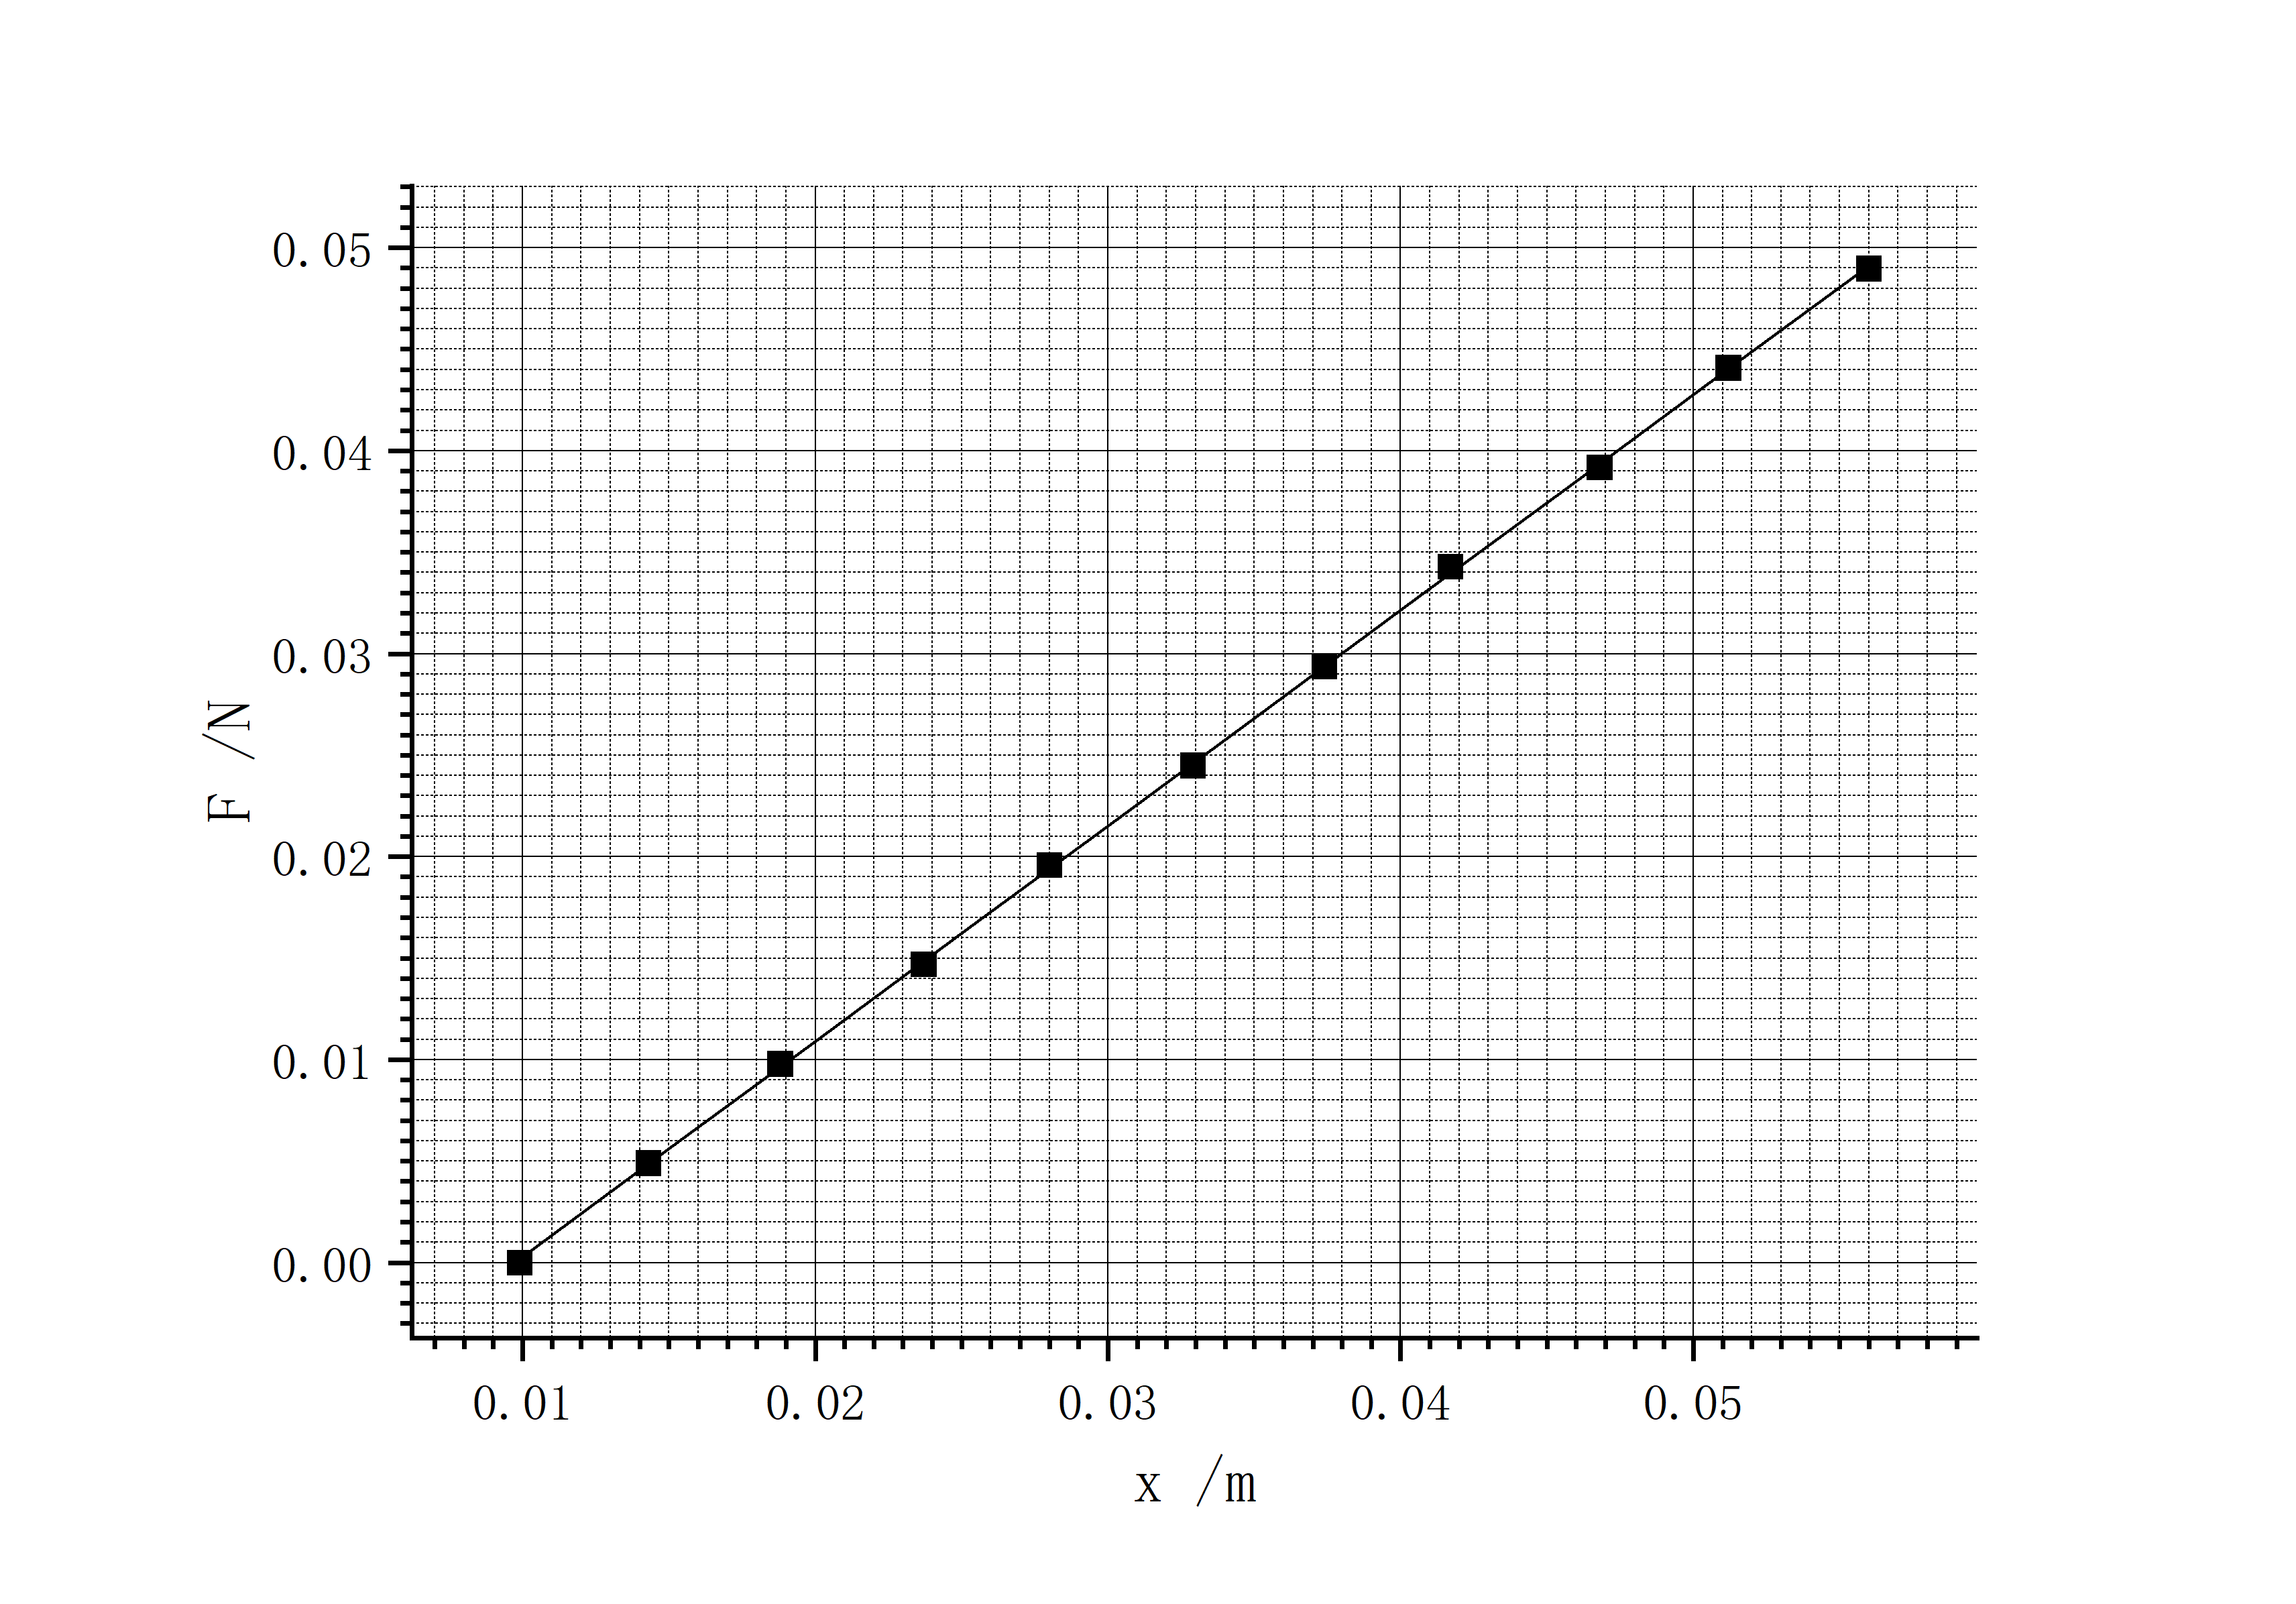
\includegraphics[width=0.8\linewidth]{sb.png}
        \caption{砝码重力与位移的实验数据图}
    \end{figure}
    由图像得到斜率约为 1 N/m ,但作图法计算的结果不够准确,故使用最小二乘法计算弹簧弹性系数。
    \subsubsection{通过最小二乘法计算弹簧弹性系数}
    \hspace{2em}
    上述数据使用Origin软件线性拟合得到:
    \begin{figure}[H]
        \centering
        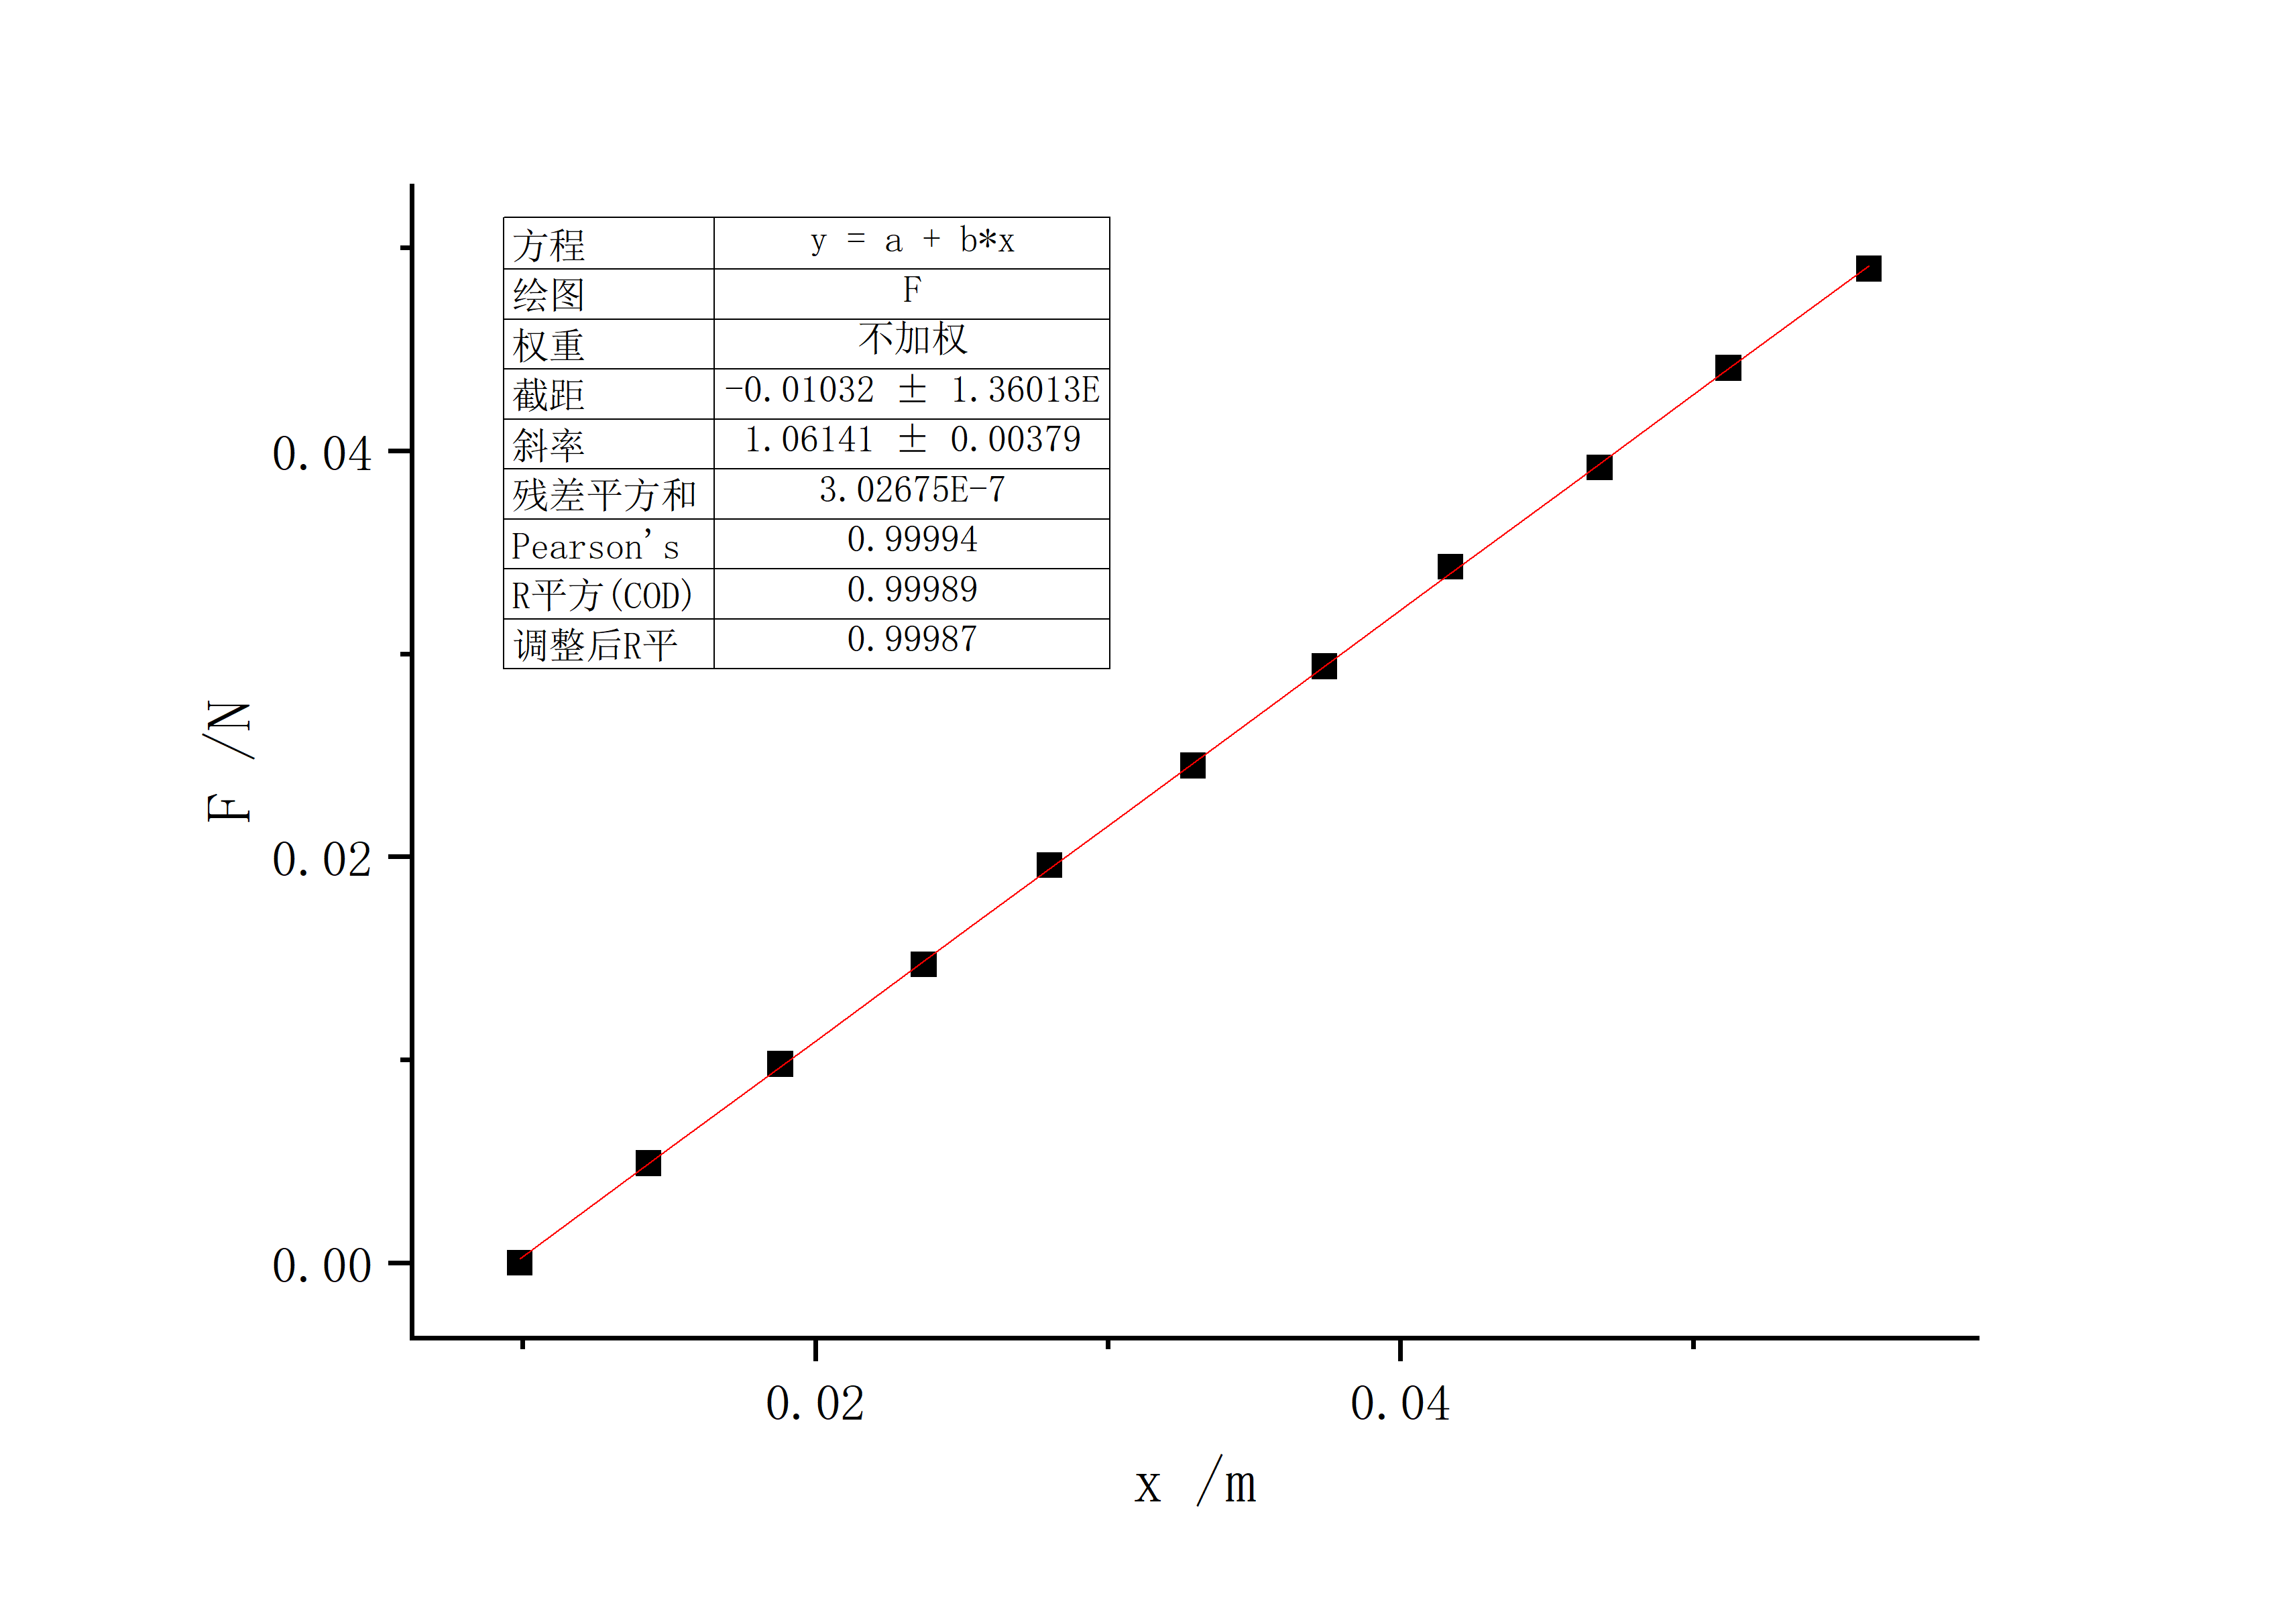
\includegraphics[width=0.8\linewidth]{1.png}
        \caption{砝码重力与位移的实验数据线性拟合}
    \end{figure}
    由图像得到斜率 1.0614 N/m ,相关系数为 0.99994 ,即弹簧的弹性系数 $k =1.0614$ N/m,其不确定度为 $\mu_k=3.8\times 10^{-3}$ N/m。故弹簧弹性系数可表示为 1.0614(38) N/m。
    \subsection{自来水表面张力系数}
    \subsubsection{金属丝直径的测量及其标准不确定度}
    \hspace{2em}
    用钢尺测量使用金属圈直径测量结果如下:
    \begin{table}[H]
        \centering
        \caption{金属圈直径测量数据}
        \begin{tabular}{cc}
            \toprule
            编号 & 金属圈直径 $d$/cm\\
            \midrule
            1 & 3.50\\
            2 & 3.45\\
            3 & 3.50\\
            \midrule
            平均值 & 3.483\\
            \bottomrule
        \end{tabular}
    \end{table}
    \hspace{2em}
    钢尺测量金属丝直径的测量模型为:
    \begin{equation}
        d=\overline{d}+d_0
        \label{eq:d}
    \end{equation}
    其中$\overline{d}$为钢尺直接读出的金属丝直径,$d_0$为钢尺的仪器误差对测量的影响,考虑到测量精度要求,测量模型中忽略了其他因素的影响。
    \par\hspace{2em}
    钢尺直接读出的摆长$\overline{d}$为A类,其不确定度$\mu_{\overline{d}}$为:
    \begin{equation*}
        \mu_{\overline{d}}=\sqrt{\frac{\sum\limits_{i=1}^{n}(d_i-\overline{d})^2}{n(n-1)}}=1.4\times10^{-4}\,\text{m}
    \end{equation*}
    \hspace{2em}
    钢尺的仪器误差$d_0$为B类正态分布,实验中用量程为 500 mm 钢尺的最大允差为 0.15 mm,其不确定度$\mu_{d_0}$为:
    \begin{equation*}
        \mu_{d_0}=\frac{\Delta_\text{尺}}{3}=5.0\times10^{-5}\,\text{m}
    \end{equation*}
    \hspace{2em}
    所以金属丝直径的不确定度为:
    \begin{equation*}
        \mu_d=\sqrt{\mu_{\overline{d}}^2+\mu_{d_0}^2}=1.5\times10^{-4}\,\text{m}
    \end{equation*}
    金属丝直径可以表示为 $d=3.483(15)\times10^{-2}$ m。
    \subsubsection{水膜破裂时弹簧伸长量的测量及其标准不确定度}
    \hspace{2em}
    使用拉脱法测量时,初始刻度 $l_0 = 0.95$ cm ,重复拉脱 5 次,水膜破裂时刻度如下:
    \begin{table}[H]
        \centering
        \caption{水膜破裂时刻度测量数据}
        \begin{tabular}{ccc}
            \toprule
            编号 & 水膜破裂时刻度 $l$/cm & 弹簧伸长量 $\Delta l$ /cm\\
            \midrule
            1 & 2.17 & 1.22\\
            2 & 2.23 & 1.28\\
            3 & 2.21 & 1.26\\
            4 & 2.15 & 1.20\\
            5 & 2.27 & 1.32\\
            \midrule
            平均值 & -- & 1.256\\
            \bottomrule
        \end{tabular}
    \end{table}
    \hspace{2em}
    弹簧伸长量的测量模型为:
    \begin{equation}
        \Delta l=\overline{\Delta l}+\Delta l_0
        \label{eq:dl}
    \end{equation}
    其中$\overline{\Delta l}$为拉脱法测量的弹簧伸长量,$\Delta l_0$为仪器误差,考虑到测量的精度要求,测量模型中忽略了其他因素的影响。
    \par\hspace{2em}
    拉脱法测量的弹簧伸长量$\overline{\Delta l}$为A类,其不确定度$\mu_{\overline{\Delta l}}$为:
    \begin{equation*}
        \mu_{\overline{\Delta l}}=\sqrt{\frac{\sum\limits_{i=1}^{n}(\Delta l_i-\overline{\Delta l})^2}{n(n-1)}}=1.9\times10^{-4}\,\text{m}
    \end{equation*}
    \hspace{2em}
    仪器读数方式类似游标卡尺,所以仪器误差$\Delta l_0$为B类均匀分布。仪器允差为 0.1 mm,其不确定度$\mu_{\Delta l_0}$为:
    \begin{equation*}
        \mu_{\Delta l_0}=\frac{\Delta}{\sqrt{3}}=5.8\times10^{-5}\,\text{m}
    \end{equation*}
    \hspace{2em}
    所以水膜破裂时弹簧伸长量的不确定度为:
    \begin{equation*}
        \mu_{\Delta l}=\sqrt{\mu_{\overline{\Delta l}}^2+\mu_{\Delta l_0}^2}=2.0\times10^{-4}\,\text{m}
    \end{equation*}
    所以水膜破裂时弹簧伸长量可以表示为 $\Delta l=1.256(20)\times10^{-2}$ m。
    \subsubsection{自来水表面张力系数及其标准不确定度}
    \hspace{2em}
    则可以计算出 $F=k\Delta l=1.333\times10^{-2}$ N ,则表面张力系数为:
    \begin{equation*}
        \sigma=\frac{F}{2\pi d}=\frac{1.333\times10^{-2}}{2\times 3.1416 \times3.483\times10^{-2}}=6.091\times10^{-2} \,\text{N/m}    
    \end{equation*}
    \hspace{2em}
    表面张力的测量模型为:
    \begin{equation*}
        \sigma=\frac{k\Delta l}{2\pi d}
    \end{equation*}
    \par\hspace{2em}
    表面张力的标准不确定度为:
    \begin{equation*}
        \begin{aligned}
            \mu_{\sigma} &= \sqrt{\left(\frac{\partial \sigma}{\partial k}\mu_k\right)^2+\left(\frac{\partial \sigma}{\partial \Delta l}\mu_{\Delta l}\right)^2+\left(\frac{\partial \sigma}{\partial d}\mu_d\right)^2}\\
            &=\sigma \sqrt{\left(\frac{\mu_k}{k}\right)^2+\left(\frac{\mu_{\Delta l}}{\Delta l}\right)^2+\left(\frac{\mu_d}{d}\right)^2}\\
            &=6.091\times10^{-2}\times\sqrt{\left(\frac{3.8\times10^{-3}}{1.0614}\right)^2+\left(\frac{2.0\times10^{-4}}{1.256\times10^{-2}}\right)^2+\left(\frac{1.5\times10^{-4}}{3.483\times10^{-2}}\right)^2}\\
            &=1.0\times10^{-3}\,\text{N/m}
        \end{aligned}
    \end{equation*}
    \par\hspace{2em}
    则自来水的表面张力系数可表示为 $6.09(10)\times10^{-2}$ N/m。
    \subsubsection{自来水表面张力系数的展伸不确定度}
    \hspace{2em}
    弹簧弹性系数$k$的自由度为$n-2=11-2=9$,金属圈直径$d$和水膜破裂时弹簧伸长量$\Delta l$的有效自由度可由测量模型\ref{eq:d}和\ref{eq:dl}得到:
    \begin{equation*}
        \begin{aligned}
            v_d&=\frac{\mu_d^4}{\frac{\mu_{\overline{d}}^4}{3-1}+\frac{\mu_{d_0}^4}{\infty}}\approx3\\
            v_{\Delta l}&=\frac{\mu_{\Delta l}^4}{\frac{\mu_{\overline{\Delta l}}^4}{5-1}+\frac{\mu_{\Delta l_0}^4}{\infty}}\approx5
        \end{aligned}
    \end{equation*}
    \par\hspace{2em}
    所以自来水表面张力系数$\sigma$的有效自由度为:
    \begin{equation*}
        \begin{aligned}
            v_{\sigma} &= \frac{\mu_{\sigma}^4}{\frac{\left(\frac{\partial\sigma}{\partial k}\mu_k\right)^4}{v_k}+\frac{\left(\frac{\partial\sigma}{\partial \Delta l}\mu_{\Delta l}\right)^4}{v_{\Delta l}}+\frac{\left(\frac{\partial\sigma}{\partial d}\mu_d\right)^4}{v_d}}\\
            &= \frac{1}{\sigma^4}\frac{\mu_{\sigma}^4}{\frac{\left(\frac{\mu_k}{k}\right)^4}{v_k}+\frac{\left(\frac{\mu_{\Delta l}}{\Delta l}\right)^4}{v_{\Delta l}}+\frac{\left(\frac{\mu_d}{d}\right)^4}{v_d}}\\
            &= \frac{(1.0\times10^{-3})^4}{\frac{\left(\frac{3.8\times10^{-3}}{1.0614}\right)^4}{9}+\frac{\left(\frac{2.0\times10^{-4}}{1.256\times10^{-2}}\right)^4}{5}+\frac{\left(\frac{1.5\times10^{-4}}{3.483\times10^{-2}}\right)^4}{3}}\\
            &\approx 6
        \end{aligned}
    \end{equation*}
    \par\hspace{2em}
    在置信区间 $P=0.95$ 下,查表得$k_{0.95}=2.45$,则自来水表面张力系数的展伸不确定度为:
    \begin{equation*}
        U_{\sigma}=k_{0.95}\mu_{\sigma}=2.45\times1.0\times10^{-3}\approx2.5\times10^{-3}\,\text{N/m}
    \end{equation*}
    所以自来水表面张力的展伸不确定度为 $2.5\times10^{-3}$ N/m,自来水表面张力的测量结果可表示为 $\sigma = (6.09\pm0.25)\times10^{-2}$ N/m。
    \subsection{洗洁精表面张力系数}
    \hspace{2em}
    使用拉脱法测量洗洁精表面张力系数。用钢刻度尺测量使用金属丝长度测量结果如下:
    \begin{table}[H]
        \centering
        \caption{金属丝长度测量数据}
        \begin{tabular}{cc}
            \toprule
            编号 & 金属丝长度 $s$/cm\\
            \midrule
            1 & 4.45\\
            2 & 4.45\\
            3 & 4.45\\
            \midrule
            平均值 & 4.45\\
            \bottomrule
        \end{tabular}
    \end{table}
    \hspace{2em}
    使用拉脱法测量时,初始刻度 $l_0 = 0.80$ cm ,重复 5 次,洗洁精膜破裂时刻度如下:
    \begin{table}[H]
        \centering
        \caption{洗洁精膜破裂时刻度测量数据}
        \begin{tabular}{ccc}
            \toprule
            编号 & 洗洁精膜破裂时刻度 $l$/cm & 弹簧伸长量 $\Delta l$ /cm\\
            \midrule
            1 & 1.04 & 0.24\\
            2 & 1.05 & 0.25\\
            3 & 1.04 & 0.24\\
            4 & 1.05 & 0.25\\
            5 & 1.05 & 0.25\\
            \midrule
            平均值 & -- & 0.246\\
            \bottomrule
        \end{tabular}
    \end{table}
    可以计算出 $F=k\Delta l=2.613\times10^{-3}$ N ,则表面张力系数为:
    \begin{equation*}
        \sigma=\frac{F}{2s}=\frac{2.613\times10^{-3}}{2\times4.45\times10^{-2}}=2.94\times10^{-2} \,\text{N/m}
    \end{equation*}
    \subsection{不同浓度洗洁精溶液的表面张力关系曲线}
    分别配置4种不同浓度的洗洁精溶液,使用拉脱法测量表面张力系数,得到的数据如下表所示:
    \begin{table}[H]
        \centering
        \caption{不同浓度洗洁精溶液的表面张力系数}
        \begin{tabular}{cccc}
            \toprule
            水与洗洁精体积比 & 初始刻度 $l_0$/cm & 破裂时刻度 $l$/cm & 弹簧伸长量 $\Delta l$/cm\\
            \midrule
            400:1 & 0.80 & 1.04 & 0.24\\
            400:1.6 & 0.86 & 1.11 & 0.25\\
            400:2.6 & 0.83 & 1.09 & 0.26\\
            400:3.6 & 0.82 & 01.09 & 0.27\\
            \bottomrule
        \end{tabular}
    \end{table}
    可以按照上述方法计算出不同浓度洗洁精溶液的表面张力系数:
    \begin{equation*}
        \begin{aligned}
            \sigma_{400:1} &= \frac{k\Delta l}{2s} =\frac{1.062\times0.24\times10^{-2}}{2\times4.45\times10^{-2}}=2.86\times10^{-2} \,\text{N/m}\\
            \sigma_{400:1.6} &= \frac{k\Delta l}{2s} =\frac{1.062\times0.25\times10^{-2}}{2\times4.45\times10^{-2}}=2.98\times10^{-2} \,\text{N/m}\\
            \sigma_{400:2.6} &= \frac{k\Delta l}{2s} =\frac{1.062\times0.26\times10^{-2}}{2\times4.45\times10^{-2}}=3.10\times10^{-2} \,\text{N/m}\\
            \sigma_{400:3.6} &= \frac{k\Delta l}{2s} =\frac{1.062\times0.27\times10^{-2}}{2\times4.45\times10^{-2}}=3.22\times10^{-2} \,\text{N/m}\\            
        \end{aligned}
    \end{equation*}
    将得到表面张力与体积比拟合:
    \begin{figure}[H]
        \centering
        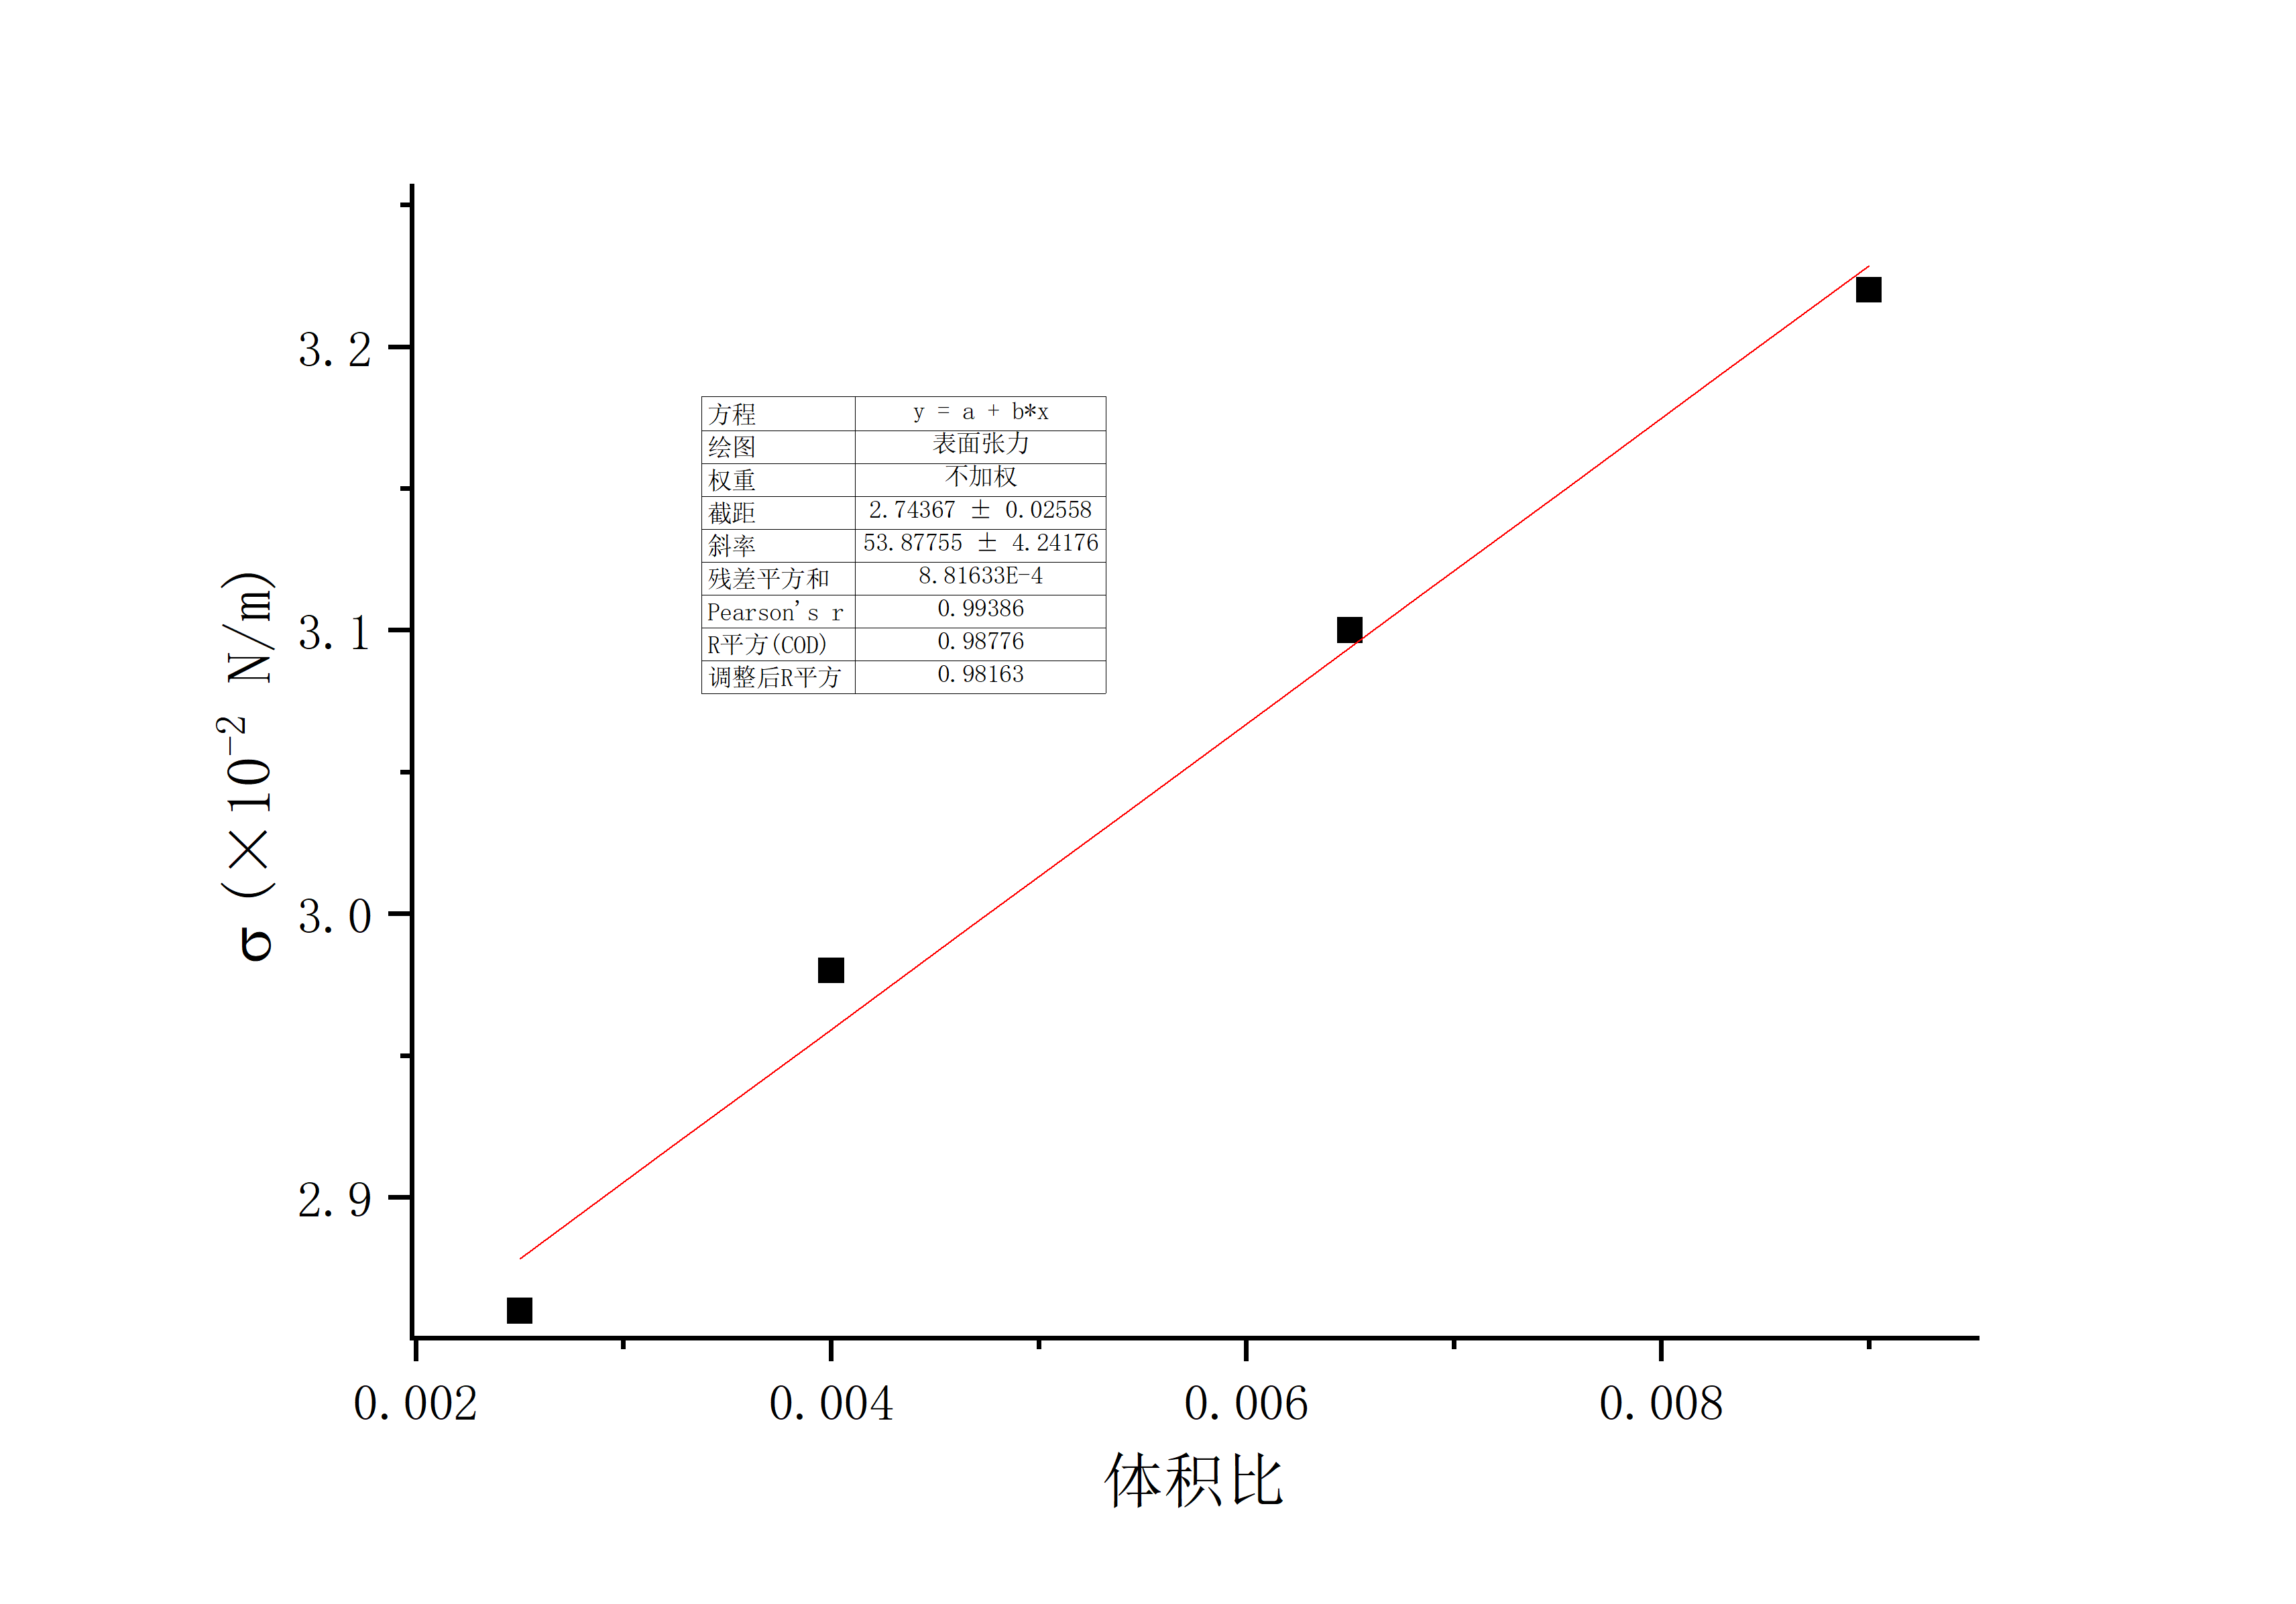
\includegraphics[width=0.8\linewidth]{2.png}
        \caption{洗洁精溶液表面张力与其浓度的线性拟合}
    \end{figure}
    \hspace{2em}
    由图可知,洗洁精溶液表面张力与其体积分数在图示浓度范围内大体呈缓慢增加趋势,但是实验中洗洁精浓度梯度过小,导致测量的弹簧伸长量间隔过小,结果可能不准确。经查阅资料得到$^{[2]}$,洗洁精溶液的表面张力在浓度较小($<0.5$ mol/L)时,表面张力随浓度增加而急剧减小,而在浓度较大时,表面张力几乎不随浓度变化,有时也随浓度增大而缓慢增加。故实验结果可能受到测量范围的限制。
    \section{结论}
    \hspace{2em}
    本文使用焦利氏秤法测量了自来水和一定浓度的洗洁精溶液的表面张力系数,其中测得水的表面张力系数为$6.09\times10^{-2}$ N/m ,一定浓度洗洁精的表面张力系数为$2.94\times10^{-2}$ N/m。并绘制了洗洁精表面张力系数随洗洁精浓度变化曲线,实验结果表明洗洁精溶液的表面张力随浓度有微弱上升趋势,但可能由洗洁精浓度区间选取不当导致。
    \section{思考题}
    \begin{enumerate}
        \item 焦利氏秤法测定液体的表面张力有什么优点?
        \par\hspace{2em}
        焦利氏秤在测量时保持下端固定不动,通过上端的位移来进行称重,因此能够迅速测量出液膜即将破裂时的力$F$。这解决了使用普通弹簧难以快速准确测出液膜破裂瞬间受力$F$的问题。焦利氏秤使用锥形弹簧,避免了因弹簧自重导致的弹性系数变化,从而提高了实验精度。焦利氏秤虽然量程范围较小,但其灵敏度高、稳定性好,锥形弹簧的弹性系数较小,使得长度读数更加准确,提升了实验精度。
        \item 焦利氏秤的弹簧为什么做成锥形?
        \par\hspace{2em}
        使弹簧均匀伸长,消除弹簧自重的影响,提高实验精度。
        \item 实验中应注意哪些地方,才能减小误差?
        \par\hspace{2em}
        实验中应注意保持焦利氏秤的三线对齐,保证弹簧的伸长量准确。应注意保护焦利氏秤的锥形弹簧,应小心拿取,并注意不要超出弹簧的弹性限度,以免弄坏弹簧。应注意小镜子不要与玻璃管摩擦,以免摩擦力影响实验结果。应注意实验用的金属圈和金属丝要先沾一下待测液体读取焦利氏秤读数,防止液珠增加的质量影响表面张力系数结果。测量清洁精的表面张力系数时先将其搅拌均匀,防止不同深度清洁精浓度不同致使的表面张力系数不同。应注意保持配件的完好,实验室玻璃器皿要小心使用,防止损坏。
    \end{enumerate}
    \section*{参考文献}
    [1]. 液体表面张力系数测定. 实验讲义. 2024\par
    [2]. 甘泉et.al.. 利用Origin双参数拟合表面张力与浓度曲线. [J]. 大学化学, 2016, 31(11): 97-100
    \newpage
    \section*{附录}
    \subsection*{老师签字的实验数据}
    \begin{figure}[H]
        \centering
        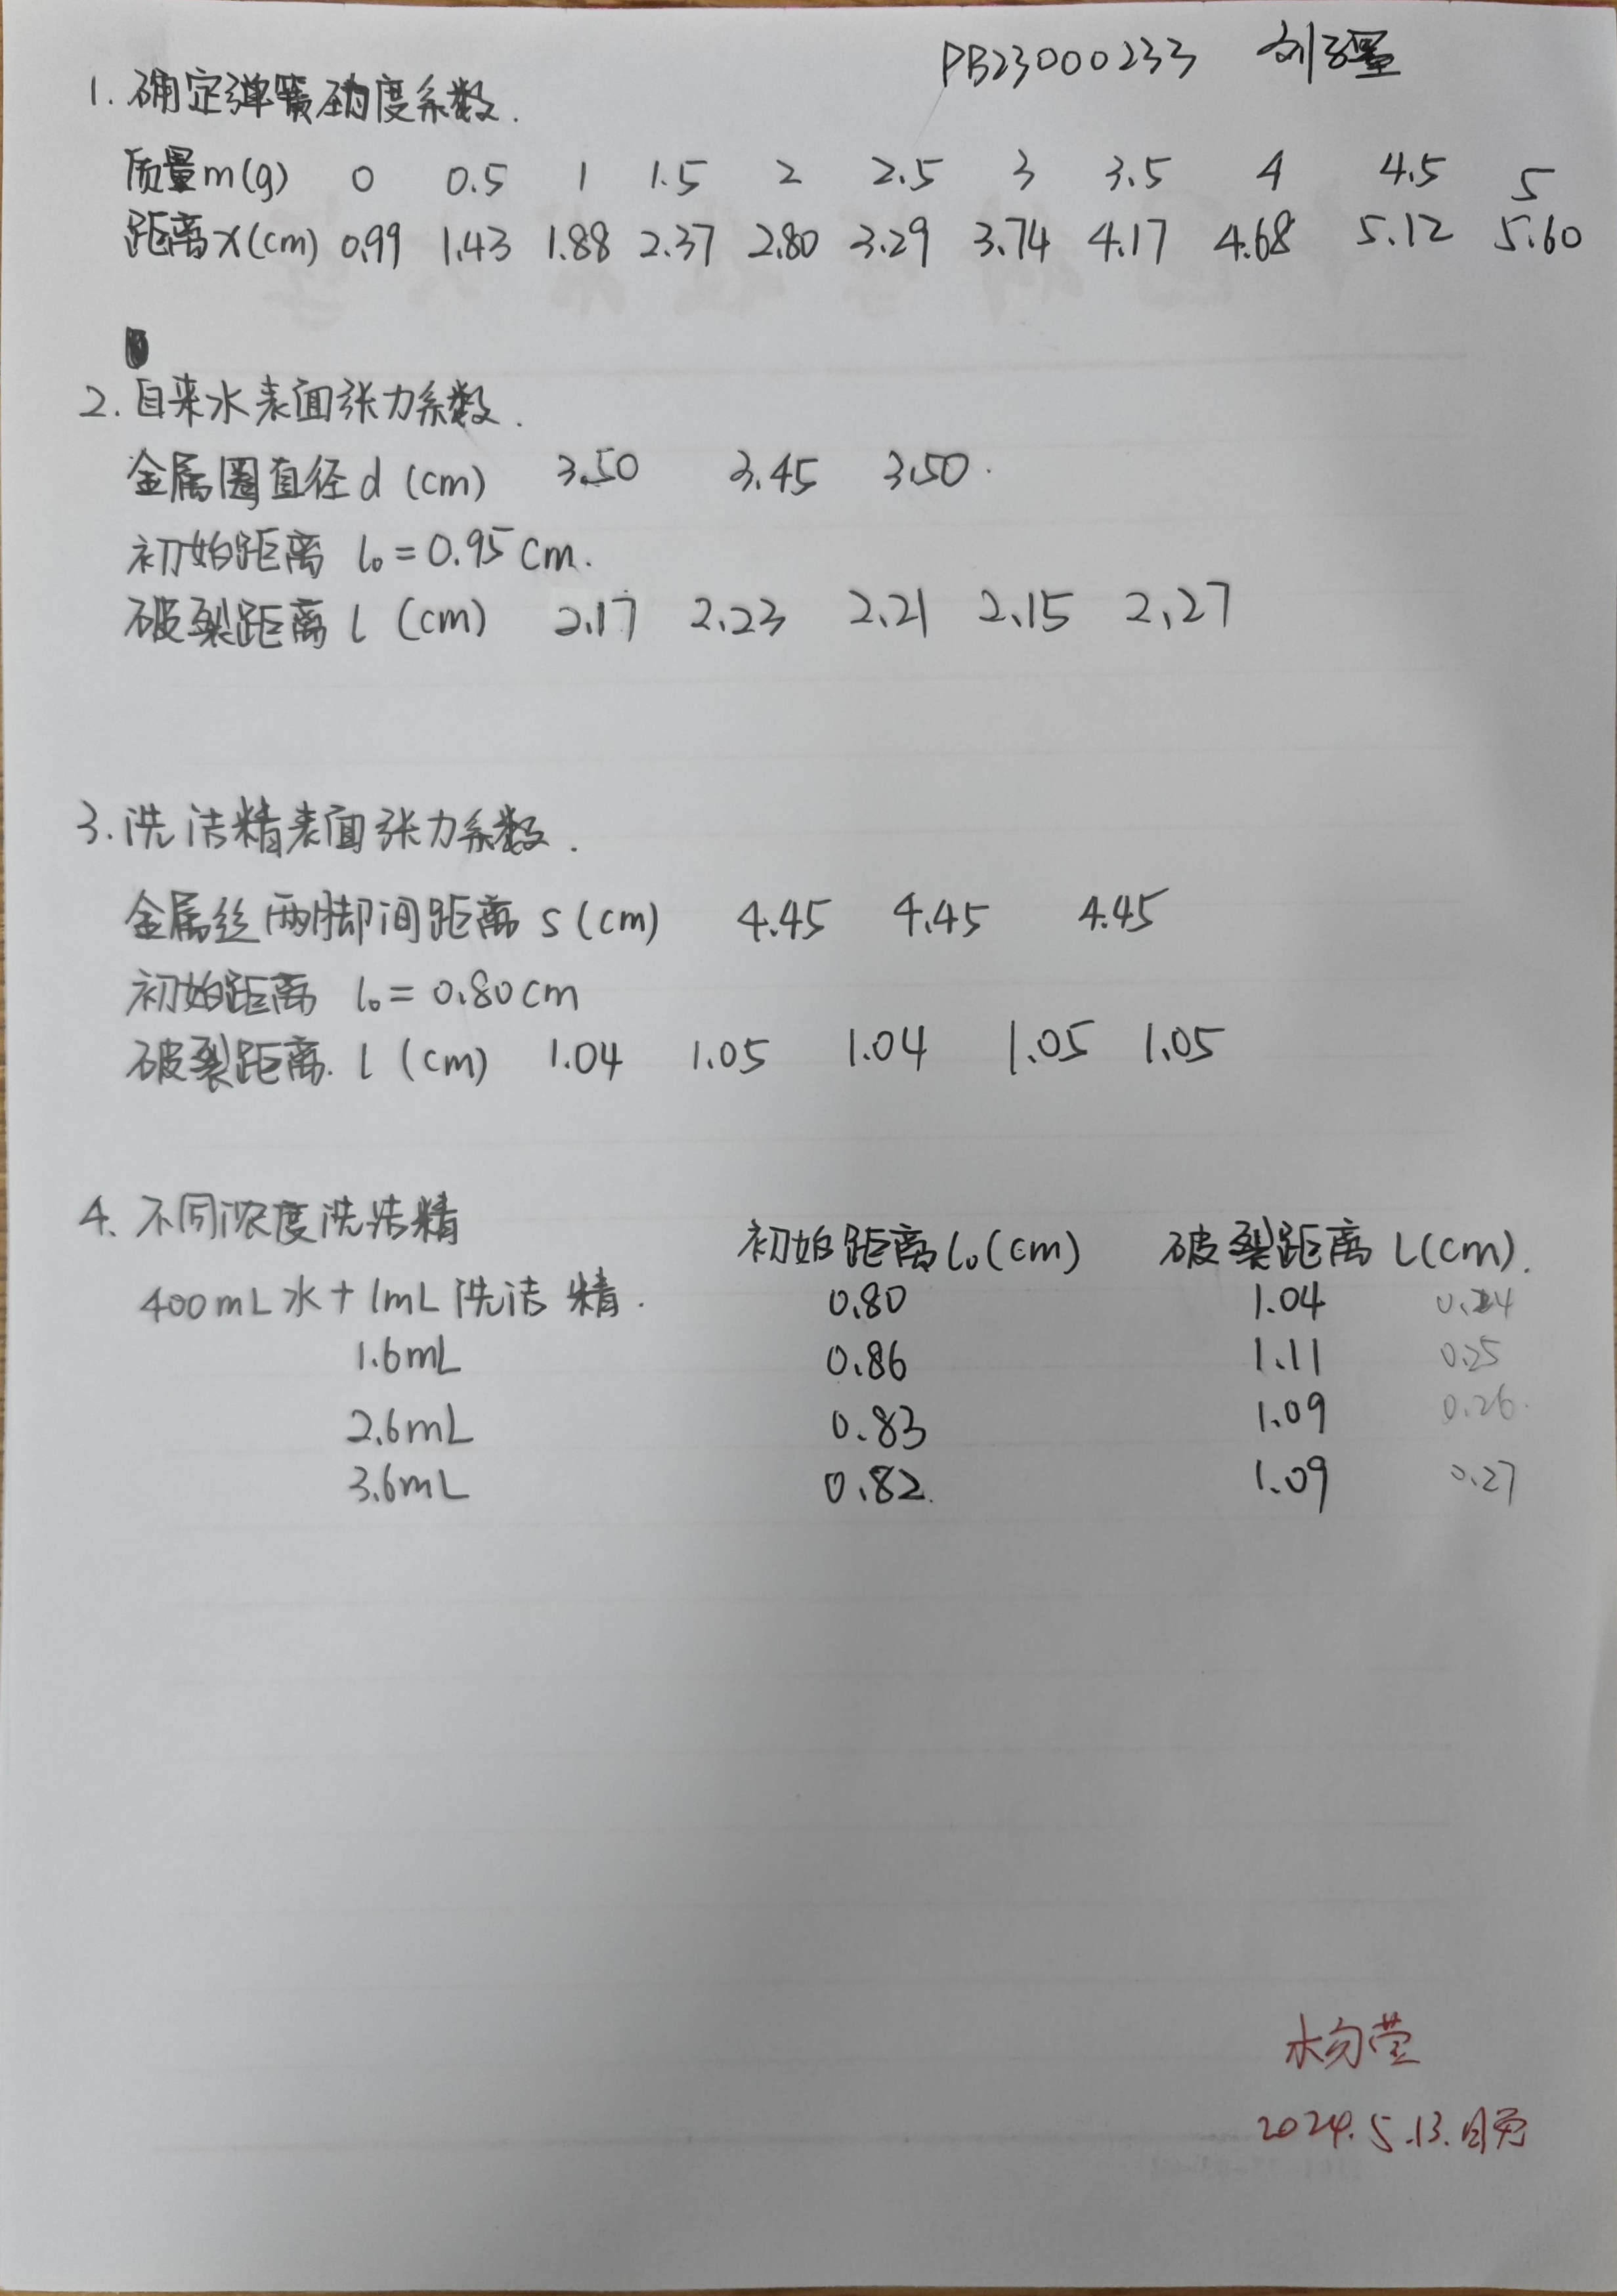
\includegraphics[width=\linewidth]{shuju.jpg}
    \end{figure}
\end{document}
